\documentclass[main.tex]{subfiles}

\begin{document}
 

\section{Validity of the model}\label{results:validity_of_the_model}

Section \ref{introduction_to_random_walks} shows that a random walk can be described by the Gaussian distribution and that it satisfies the diffusion equation as well as deriving the diffusion equation from a random walk. 
Mathematically these models are considered equivalent in the limit of sufficiently many walkers. 
This limit is defined by the time step as 
\begin{equation}
 N \geq \frac{1}{\Delta t^2}
\end{equation}
Figure \ref{combined_BE1d:convergence} verifies that given a sufficient amount of walkers, the convergence in time is unaffected by the walkers. 
Thus supporting the claim that the models are equivalent, and that they can be combined in a meaningful way. \\

For all practical purposes, however, the demand for walkers is too high, and will generally only be met for verification purposes. 
This is no problem, since the models were combined to study effects from both length scales, which would not be meaningful to study if the demand for walkers is met. 

In other words, the model converges to the continuum model in the limit of sufficient walkers, but this limit is seldom met.

% The results of the testing done in the Analysis-chapter, particularly the convergence tests based on varying the conversion-factor, Hc, to exceed the expected numerical error arising from the scheme itself based on equation \ref{}, suggest that the implementation of our model is correct. 
% The mathematics overlap, as we have seen in chapter \ref{}, and if we introduce enough walkers there seems to be no difference between adding an area on the mesh where random walks solve the equation, and not doing so. 

\section{Diffusion times into spines}

Craske et.al. suggest that the neck of spines act as diffusion barriers which slow down, but don't completely stop the diffusion of PKC$\gamma$ into spines. 
The function of this barrier is a bit unclear, but the presence of it is undisputed. 
In their measurements they found a delay of around $5-10$ seconds from elevated concentration levels in the dendrite until a similarly elevated concentration level occurred in spines with necks longer than $0.5\mu$m. 
Using parameter values which resemble the values found in actual (rodent) neurons and neurites in the developed software, the observed delay-times have been recreated. 
Figure \ref{results:spine_diffusion_stats} shows plots of the observed diffusion times into spines. 
This figure shows a clear trend for longer diffusion times as the neck length of the spine increases. 
Figure \ref{results:boxplot_relative_diffusiontime_long_neck} further support this claim and implies the average diffusion time for PKC$\gamma$ into long necked spines to be of accordance to the results from Craske et.al.
Seeing as there are no additional complexities added to the random walk model we can assume that the spine neck does in fact function as a diffusion barrier.

\begin{figure}[H]
 \centering
\begin{subfigure}[b]{0.48\textwidth}
 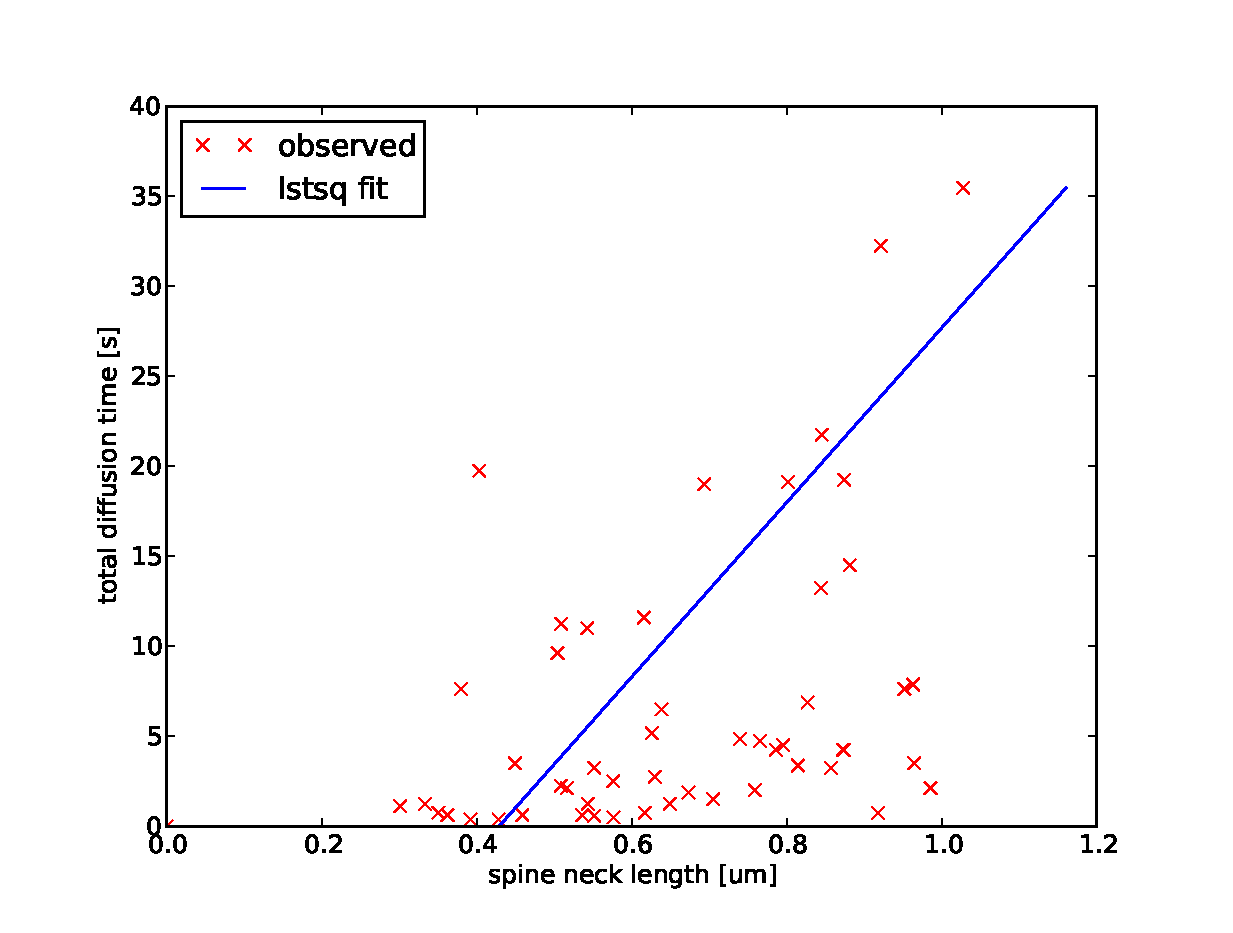
\includegraphics[width=\textwidth]{Figures/spine_stats_fulltime_nl.eps}
 \caption{Absolute diffusion times.}
 \label{results:spine_diffusion_stats:fulltime}
 \end{subfigure}
 \begin{subfigure}[b]{0.48\textwidth}
 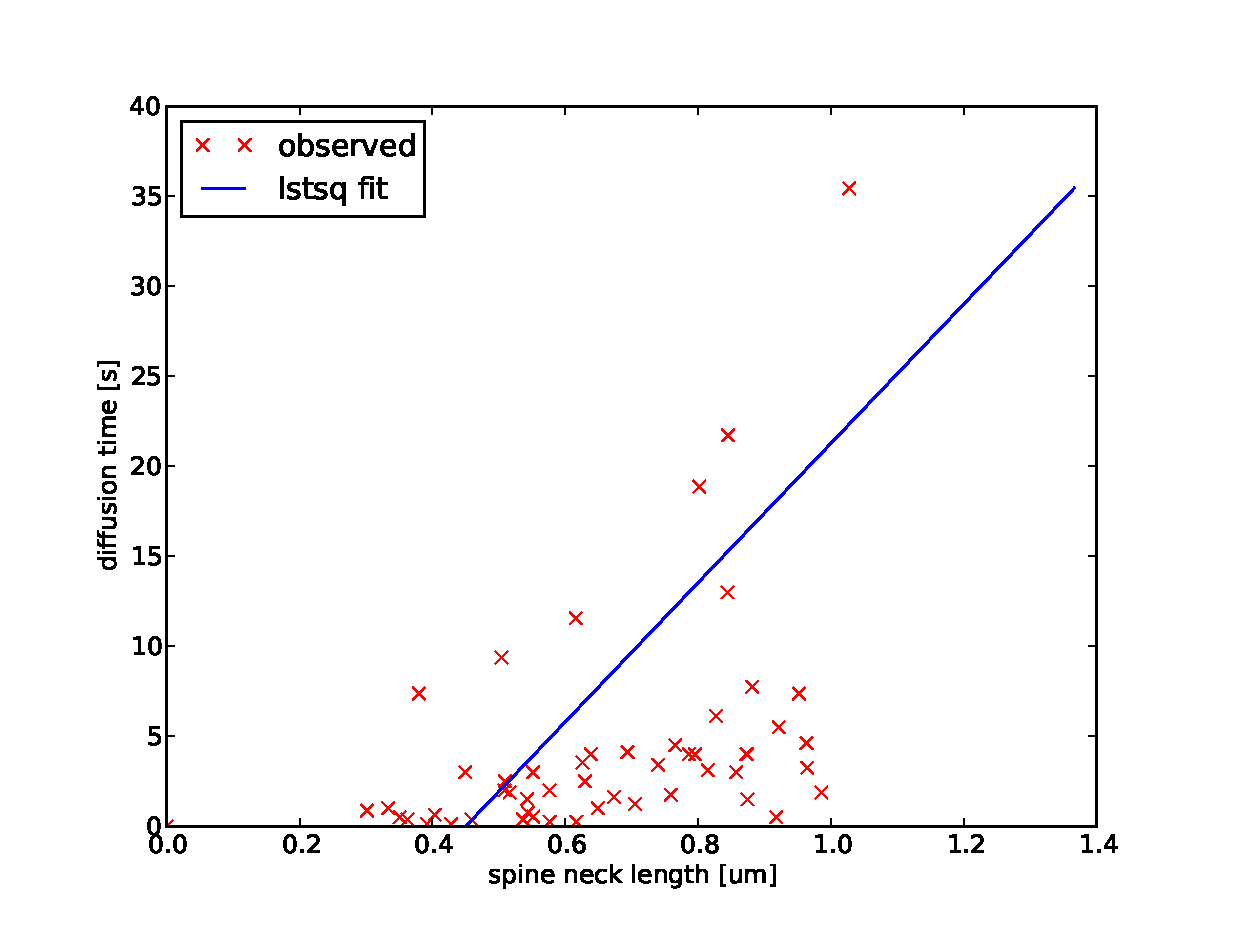
\includegraphics[width=\textwidth]{Figures/spine_stats_reltime_nl.eps}
 \caption{Relative diffusion times.}
 \label{results:spine_diffusion_stats:reltime}
\end{subfigure}
\caption[Diffusion times with least squares fit]{Absolute (a) and relative (b) diffusion times into spines. The lines represent a least squares fit of the results. This least squares fit should have been done after removing outliers and should have an expression written out somewhere.}
\label{results:spine_diffusion_stats}
\end{figure}

\begin{figure}[H]
 \centering
 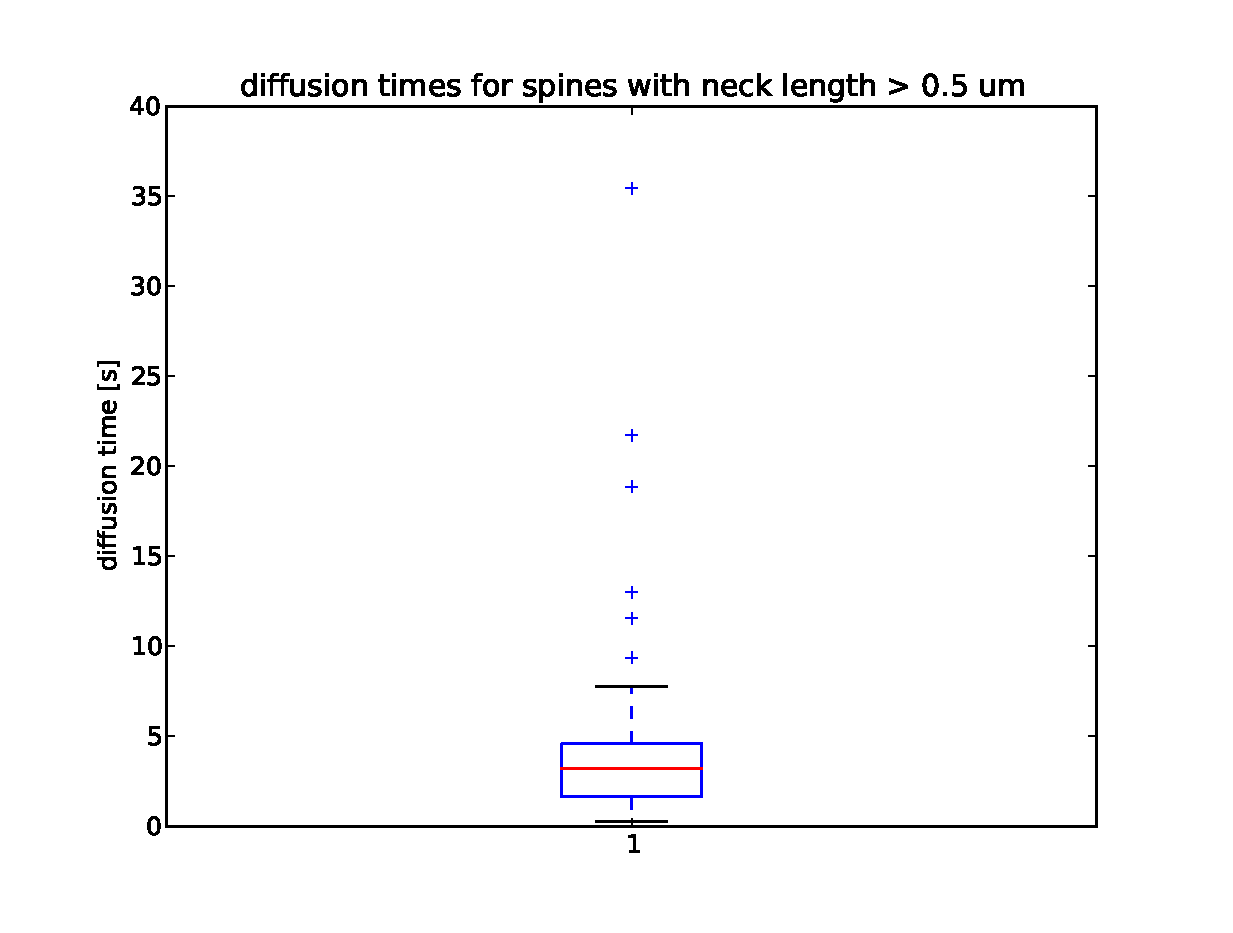
\includegraphics[scale=0.5]{Figures/spine_stats_boxplot_reltime_longneck.eps}
 \caption[Diffusion time for long necked spines]{Boxplot of the relative diffusion times (time between elevated concentration in dendrite and elevated concentration in spine head) into spines with necks longer than $0.5\mu$m. Similar studies were done by Crase et.al. and found diffusion time (unclear whether relative or not) to be somewhere around 5-10 seconds.}
 \label{results:boxplot_relative_diffusiontime_long_neck}
\end{figure}

Through the simulations it became apparent that there must be some sort of limiting factor which limits the number of PKC$\gamma$ particles that are let into the spine. 
In real life this is achieved by a concentration gradient which tends to zero (or negative values) meaning that no particles will diffuse into the spine after it is ``filled'' up. 
A random walker will not feel this concentration gradient unless it is explicitly told so. 
The alternative solution then, is to reduce the probability for particles to diffuse into a spine for each particle that get caught in the spine head by some reasonable factor. 


\end{document}